%%%% ijcai19-multiauthor.tex

\typeout{IJCAI-19 Multiple authors example}

% These are the instructions for authors for IJCAI-19.

\documentclass{article}
\pdfpagewidth=8.5in
\pdfpageheight=11in
% The file ijcai19.sty is NOT the same than previous years'
\usepackage{ijcai19}

% Use the postscript times font!
\usepackage{times}
\usepackage{soul}
\usepackage{url}
\usepackage{graphicx}
\usepackage[hidelinks]{hyperref}
\usepackage[utf8]{inputenc}
\usepackage[small]{caption}
\usepackage{graphicx}
\usepackage{amsmath}
\usepackage{booktabs}
% installez ce package -> sudo apt-get install texlive-science
\usepackage[ruled,vlined]{algorithm2e}
\urlstyle{same}
\usepackage{biblatex}
\addbibresource{ijcai19.bib}

% the following package is optional:
%\usepackage{latexsym} 

% Following comment is from ijcai97-submit.tex:
% The preparation of these files was supported by Schlumberger Palo Alto
% Research, AT\&T Bell Laboratories, and Morgan Kaufmann Publishers.
% Shirley Jowell, of Morgan Kaufmann Publishers, and Peter F.
% Patel-Schneider, of AT\&T Bell Laboratories collaborated on their
% preparation.

% These instructions can be modified and used in other conferences as long
% as credit to the authors and supporting agencies is retained, this notice
% is not changed, and further modification or reuse is not restricted.
% Neither Shirley Jowell nor Peter F. Patel-Schneider can be listed as
% contacts for providing assistance without their prior permission.

% To use for other conferences, change references to files and the
% conference appropriate and use other authors, contacts, publishers, and
% organizations.
% Also change the deadline and address for returning papers and the length and
% page charge instructions.
% Put where the files are available in the appropriate places.

\title{Entrainement d'un agent virtuelle par Q-learning pour le jeu Snake}

\author{
Samuel Ferron\and
Jean-Frédéric Fontaine\and
Noboru Yoshida
\affiliations
Department de génie logiciel, Polytechnique Montréal, Canada\\
\emails
\{samuel.ferron, jean-frederic.fontaine, noboru.yoshida\}@polymtl.ca
}

\begin{document}

\maketitle

\begin{abstract}
This short example shows a contrived example on how to format the authors' information for {\it IJCAI--19 Proceedings} using \LaTeX{}.
\end{abstract}

\section{Introduction}

Noboru

\section{Revue de la littérrature}
 
Noboru

\section{Explication du jeu Snake }
Le jeux Snake consiste en un environnement fermé 2D dans lequel une représentation simplifiée (en pixel) d'un serpent doit atteindre un point, qui consiste à de la nourriture, afin d'accumuler des points. Lorsque le point est atteint le serpent augmente de taille. Si le serpent entre en contact avec lui-même ou encore avec une paroie de l'environnement; la partie est termimée. Ainsi, le jeux devient de plus en plus difficile étant donné que la longueur du serpent augmente et la capacité de celui-ci à faire certains déplacement diminue. Certaines versions du jeux accélèrent aussi la vitesse de déplacement du serpent en plus de sa taille. Dans notre implémentation, nous n'avons pas ajouté cette fonctionnalité car la vitesse à laquelle l'agent prend une décision ne nous importe peu (l'horloge d'un processeur est beaucoup plus rapide que la vitesse maximale à laquelle un humain peut jouer), c'est plutôt la qualité de la décision qui nous importe. La figure 1 montre l'interface de notre jeux de snake. À gauche de la figure on témoigne d'un Snake en début de parti et à droite après quelques minutes de jeux. 
\begin{figure}[ht]
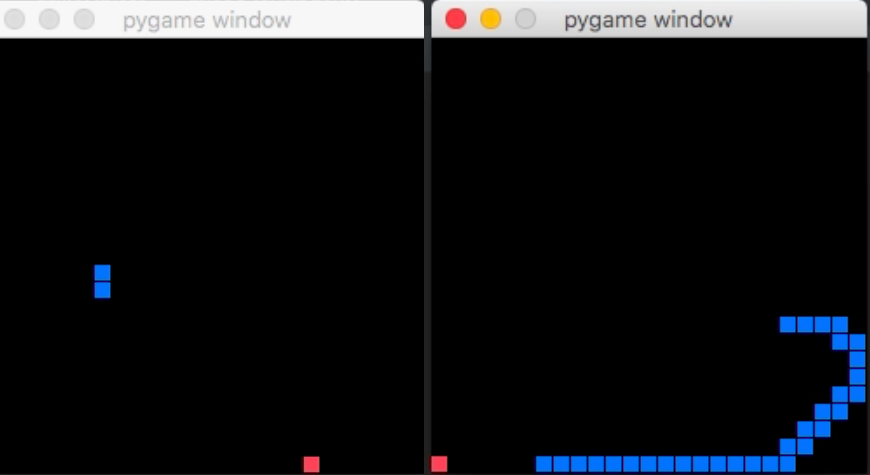
\includegraphics[width=\linewidth]{snake.png}
\caption{Snake qui augmente sa taille en atteignant la cible.}
\label{fig:Snake}
\end{figure}

\section{Q-Learning : Explication théorique  }
Généralement, les algorithmes d’apprentissages machines dépendent d’un grande quantité de donnée qui ont été étiquetées à la main afin de pouvoir faire des prédictions de qualité. Cependant, dans le contexte de l'apprentissage par renforcement, l’idée est plutôt de permettre à un l’algorithme, c’est-à-dire un agent, d’apprendre par lui-même les règles qui définissent le succès ou l’échec d’une tâche quelconque.\linebreak

Afin de se faméliariser avec l'algorithme de Q-learning nous avons entrainé un agent à jouer au jeux Snake selon  une politique de renforcement relativement simple.Pour ce faire, nous avons émulé l'expérience réalisé par Mnih et al. \cite{DBLP:journals/corr/MnihKSGAWR13}. Dans cette procédure, les chercheurs ont entrainé un agent virtuel à jouer à plusieurs jeux Atari. L'agent consiste en un réseau de neuronne à convolution qui reçoit comme entré la réprésentation visuelle du jeux, c'est-à-dire une image 210X160 pixels RGB. L'agent est ensuite entrainé par l'algorithme de Q-Learning selon une procédure de renforcement ( i.e récompense). En s'inpirant de cette approche et du blog de Comi \cite{comi_2020}, nous avons mis en place une procédure similaire avec la seule différence que nous fournisons à l'agent une représentation simplifié de l'état de la partie, non pas une image.  Plus précisément, considérons un agent virtuelle qui intéragit avec l'environnement $\xi$ (i.e le Snake), dans notre cas, un environnement 2D fermé, au Snake
et à la nourriture que celui-ci doit atteindre afin de recevoir une récompense. À chaque époque temporelle, c'est-à-dire, à chaque nouveau déplacement du Snake, l'agent doit choisir une action  $\alpha_t$ au temps $t-1$  parmis l'ensemble d'action légal $\Delta  = \{1, ..., K\}$. Une fois l'action choisie, celle-ci est exécutée. Cette action a pour effet de modifier l'état interne de la partie. Afin d'éxécuté une nouvelle action au temps $t$, nous fournissons à l'agent le nouvel état ainsi qu'une récompense si son action au temps $t-1$ le méritait. Dans notre approche, nous fourinissons à l'agent une représentation simplifiée de la partie basé sur l'éminence d'un danger et la direction de la nourriture du snake. Nous considérons donc pour le temps $t-1$ un vecteur qui décris l'état de la partie et l'action qui a été prise pour cet état $s_t = x_1, \alpha_1$. La prochaine action de l'agent pour le temps $t$ sera basé sur le vecteur $s_t$. Le but de l'agent est donc de choisir une nouvelle action afin de maximiser une récompense future (ou minimiser les renforcements négatifs). Afin d'entrainer l'agent, nous définissons la fonction d'action optimal $Q^*(s,a)$ qui consiste au renforcement maximal attendu en suivant n'importque qu'elle stratégie après avoir vue un état $s$ et avoir pris une action $\alpha$, c'est-à-dire que $Q^*(s,a)= max_\pi 	\mathrm{E} \{R_t | s_t = s, \alpha_t = \alpha, \pi\}$ où $\pi$ est une politique qui associe un état de la partie à une action.  La fonction d'action optimal obéit une identité importante appelé équation de \textit{Bellman}. L'idée derrière cette équation est la suivante; si la valeur optimale de $Q^*(s',a')$ à l'état $s'$ était connue pour toute les actions possibles $\alpha'$, alors la stratégie optimale est de choisir l'action $\alpha'$ qui maximise le renforcement attendu pour $r + \gamma Q^*(s',a')$. Dans le contexte de l'apprentissage par renforcement, nous pouvons cherché une solution qui approxime $Q^*$ en incorporant dans un réseaux de neuronne la fonction 

$$NewQ(s,a) = Q(s,a)  + \alpha [\ R(s,a) + \gamma maxQ{'} (s{'},a{'}) - Q(s,a) ]\ $$

Où $NewQ(s,a) $ correspond à la nouvelle récompense attendue au temps $t$, $Q(s,a)$ à la récompense approximée au temps $t-1$ correspond à l'action prise au temps $t-1$, $\alpha$ au taux d'apprentissage, $R(s,a)$ à la récompense donnée pour cette action, $\gamma$ au "Discount rate" (constante souvent initialisé à .99) et $maxQ{'} (s{'},a{'})$ correspond au la valeur maximal de la récompense attendue pour toutes les actions possibles ( qui correspond à la sortie du réseau de neuronnes). Ainsi, nous appliquons cette formule de façon itérative et nous optimisons la fonction de perte de type MSE (Mean Squared Error)  $L( \theta_{i}) = [\ y_{i} - Q(s,a; \theta_{i})^{2} ]\ $. Autrement dis, l'agent estime la meilleur action a prendre selon la récompense attendue. À la prochaine iétration, on réestime la même action selon le même état en sachant la récompense que cette action a rééellement donnée. On calcule la différence entre l'estimation et la récompense réellement atteinte (la fonction de perte) puis on ajuste les poids à l'aide de la descente du gradiant. De plus, pour toute les partie, nous enregistront en mémoire chaque actions prises par l'agent ainsi que les états et les récompenses obtenues. À la fin de chaque partie, nous prenons un échantillon qui représente autant les actions qui ont provoquées un renforcement positifs que les actions qui ont provoquées un renforcement négatifs. Aisni, nous procédons à une deuxième phase d'apprentissage entre les parties en fonctions de ces échantillons. Ceci permet à l'agent d'être proportionnelement entrainé sur des situations qui pourraient arrivé moins souvent (e.g trouvé la nourriture). 

Il suffit ensuite de remplacer la nouvelle valeur récompense attendu au temps $t$ pour la récompense

\subsection{Algorithme d'apprentissage}



Ainsi, 
\section{Explication de notre implémentation}

L’implémentation proposée peut se diviser en trois parties distinctes: Le jeu, l’agent et le contrôleur.

Premièrement le jeu. L’objectif du projet est d’entraîner un DQN sur le jeu classique Snake, il nous faut donc une forme du jeu avec laquelle nous aurons accès à son état et à son contrôle. Nous avons choisis de recréer le jeu en Python à l’aide de la librairie PyGame, ce qui nous permet d’avoir un accès direct aux éléments nécessaire. En premier lieu, il faut définir l’état qui sera utilisé pour entraîner l’agent. L’état représente l’environnement dans lequel le serpent se retrouve. Il représente aussi l’entrée de notre modèle. Dans notre cas, l’état aura la forme d’un vecteur avec 11 valeurs booléennes qui indiquent les situations suivantes:

\begin{itemize}
	\item La nourriture est à gauche, en face, à droite ou en arrière du serpent.
	\item Il y a un danger imminent à gauche, en face ou à droite du serpent.
	\item La direction du serpent (gauche, haut, droite ou bas).
\end{itemize}

Les actions possibles que nous pouvons donner au jeu sont aller à gauche, continuer dans la même direction ou aller à droite.

Deuxièmement, l’agent. L’agent est l’entité qui contient le modèle d’apprentissage et qui dicte les actions à prendre selon un état donné. Nous utilisons un réseau de neurones profond. Il contient trois couches cachées avec 120 neurones avec activation de type ReLU suivit d’une couche de finale de type Softmax a trois sorties, une pour chaque action. L’agent est entraîné à chaque pas que le serpent fait et conserve une mémoire qui lui permet un entraînement en lot entre les parties. L’entrainement d’un pas considère l’état original du pas, l’action prise, l’état actuel ainsi que la récompense obtenue suite à l’action. Le système de récompense est simple; si le serpent perd, la récompense est mise à -10. Si le serpent mange, la récompense est mise à 10.

Troisièmement, le contrôleur est ce qui orchestre l'interaction entre le jeu et l’agent. Ce code implémente l’algorithme Deep Q-Learning. Nous utilisons une variable, epsilon, qui permet d’effectuer une action aléatoire selon une probabilité. Cette variable dégrade entre chaque partie et promue l’exploration dans les premières époques de l’entraînement. Le programme se déroule comme suit:

\begin{algorithm}
\caption{Séquence d'entraînement de l'agent}
\KwResult{Un agent intellligent entraîné}
initialisation\;
\For{i in epochs}{
	initialistion du jeu\;
	entraîner l'agent avec sa mémoire\;
	\While{not done}{
		Prendre l'état actuel\;
		Prédire les récompenses associé a chaque actions possible par le modèle\;
		Effectuer l'action qui favorise la meilleure récompense\;
		Prendre le nouvel état\;
		Calculer la récompense selon le nouvel état\;
		Comparer la récompense obtenu avec celle prédite (fonction de perte)\;
		Entrainement du modèle par descente du gradiant avec Q-learning\;
	}
}
\end{algorithm}

Le résultat est un agent entraîné selon un nombre d'époques (parties).

\section{Résultats}

La configuration choisie pour l'entraînement est une grille de jeu 20 par 20 où chaque fruit mangé donne un point. L’agent as été entraîné pendant 200 époques (parties) avec une valeur epsilon = 1 / 100 (disparut après 100 parties) en laissant une probabilité de 1\% de faire une action aléatoire. Les figures suivantes représentent deux métriques intéressantes pour visualiser la progression de l'agent.

\begin{figure}[ht]
	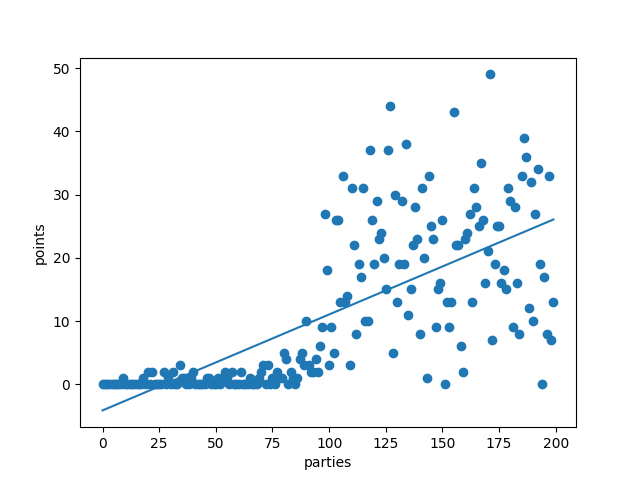
\includegraphics[width=\linewidth]{scatter_score_200_games.png}
	\caption{Nuage de points du pointage par rapport au nombre de parties jouée.}
	\label{fig:Snake}
\end{figure}

La première figure montre le pointage par rapport au nombre de parties jouées. On peut voir que le pointage lors de la période d’exploration reste bas. C’est expliqué parce que le serpent effectue des actions aléatoires et se rend rarement à la nourriture. On voit toutefois qu’il apprend correctement et obtient de bons scores avec une moyenne de 10.965 points par parties et un score maximal de 49 points. Une limitation du modèle est que l’état utilisé ne permet pas de représenter si le serpent s’enroule sur lui même. Cette situation arrive plus souvent lorsque le score devient haut et est une raison pourquoi le score semble stagner après un certain nombre de parties. La probabilité d’action aléatoire reste présente pendant tout l'entraînement, ce qui peut causer certaines anomalies, mais reste important pour éviter de tomber dans un états de boucle infinie.

\begin{figure}[ht]
	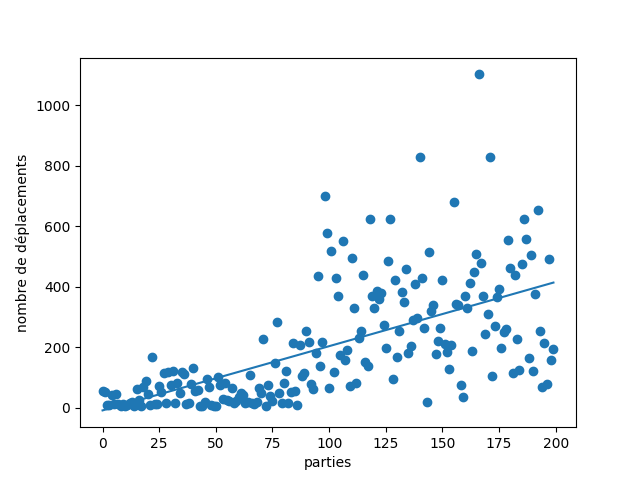
\includegraphics[width=\linewidth]{moves_per_game_200.png}
	\caption{Nuage de points du nombre de déplacements par rapport au nombre de parties jouée.}
	\label{fig:Snake}
\end{figure}

La deuxième figure présente le nombre d'actions par rapport au nombre de parties jouées. On remarque que cette métrique semble corrélée avec la métrique de pointage. L'agent se concentre sur le pointage, c'est-à-dire qu'il tente toujours de se rapprocher de la nourriture avant tout.

En observant l'agent jouer, il est évident que son comportement est limité. L'agent peut seulement interpréter les dangers imminents et a tendance à s'entreméler sur lui même et perdre. Cette limitation cause un plateau que l'agent ne semble pas surpasser avec un entrainement plus long.


Pour une meilleure vue d'ensemble, 
\href{https://www.youtube.com/watch?v=HNeuuXA3Flg&feature=youtu.be}{voici un lien vers une capture d’un entraînement pour visualiser le comportement du serpent}
ainsi
\href{https://github.com/Adrimeov/snakeAI}{qu'un lien vers le répertoire Git avec le code source de l'implémentation proposée.}


\section{Améliorations possible}

Une difficultée observée était que le modèle semblait seulement apprendre à survivre. Nous avons expérimenté de différentes façons pour altérer ce comportement. Par exemple, nous avons modifiés le système de récompenses afin de bonifier l’agent lorsque le serpent mange ou simplement ajouté une récompense positive lorsqu’il se déplace sans perdre. Le comportement ne semblait pas changer selon les récompenses. Le problème apparaissait à cause de l’entraînement qui est effectué avec la mémoire entre chaque époques. Lors des premières parties, le serpent réussissait rarement à manger donc sa mémoire était remplie d’états où les récompenses sont nulles ou négatives. Il apprenait donc seulement à se déplacer et éviter les dangers. La solution choisie était de sauvegarder un ensemble équilibré de mémoires qui représentent les différentes récompenses. Après avoir fait ce changement, le serpent vite compris à gérer les différentes solutions.

La solution proposée est très spécifique au jeu Snake et beaucoup de changements seraient nécessaires si nous voulions l’adapter pour un autre jeu. L’état donné à l’agent, soit la dimension de l’entré du modèle, n’est valable que pour ce jeu et nous pouvons dire la même chose du vecteur d’action. Une solution possible pour rendre l’état générique serait d’utiliser l’image du jeu comme entrée. Cette technique permet de ne pas avoir à extraire manuellement un vecteur qui représente l’environnement du joueur. Sinon, il serait possible d’expérimenter avec des réseaux convolutionnels où d’autres techniques plus intéressantes qu’un simple réseau de neurones profond.

\section{Conclusion}

JF

\printbibliography
\end{document}

